Our algorithms must be able to handle big data set to some extent, for example we can easily think of a scenario where each core has to sort half a gigabyte of data, and we are using 256 cores; the total memory used, among the whole system, is 128 gigabytes of data.
At least the first phases of any algorithm (before data is fully distributed), and the last phases (while data is getting gathered) will have for sure to support datasets that cannot fit in principal memory, and will be forced to run their computations on some files allocated in secondary memory.

\begin{wrapfigure}{r}{0.3\textwidth}
  \begin{center}
    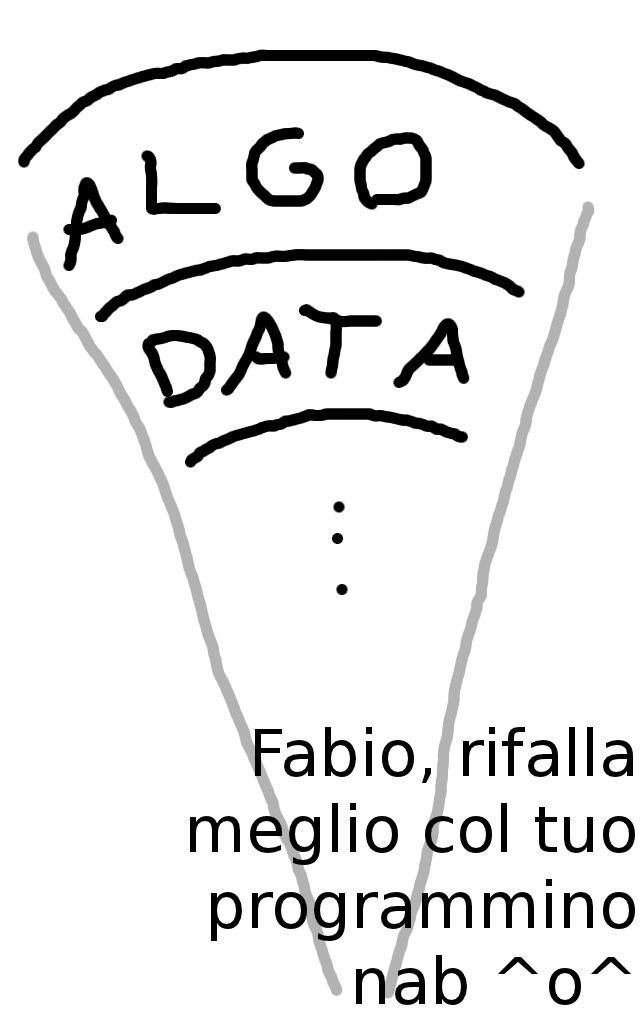
\includegraphics[width=0.28\textwidth]{datalayer.png}
  \end{center}
  \caption{Our abstract model}
\end{wrapfigure}

At this porpose we decided to add a further abstraction layer below the actual sorting algorithm: we decided to introduce a new data structure called \texttt{Data} that represents a dataset indipendently on its form or position: it can represent both an array allocated on principal memory or a file allocated on the hard disk, and it has been thought to be able to represent even other kind of data representation (eg: a compressed dataset). The sorting algorithm, which is our higher abstraction level, doesn't need to know about how or where \texttt{Data} is allocated, and use it in a transparent way.
We needed to write some kind of run-time support for this level, which is logically placed just below the algorithm sorting: since we want to save the algorithm from actually care about how Data is allocated, it needs to use some functions that will take care of it exposing a data-independent signature. Our rule of thumb is that all and only the functions logically placed at this abstraction level are the only ones actually working with a \texttt{Data} object (ie: accessing its field directly or indirectly) and vice-versa.
Functions at this abstraction level will one (or more) \texttt{Data} object, will see wether it's allocated on primary or secondary memory, and according to this they'll run some data-dependent codes, optimized for the medium where the \texttt{Data} object is allocated.

\subsubsection*{TODO}
Di che altro c'e' da parlare?
\begin{itemize}
	\item{Come funziona piu' nel dettaglio il framework e/o gli algoritmi tenendo conto del data?}
	\item{Come sono implementati (in via generale/con quale logica -- e/o anche nello specifico) gli algoritmi al livello data?}
	\item{Il fatto che abbiamo dovuto astrarre MPI?}
	\item{DOBBIAMO far capire che sta cosa non e' banale, che c'e' costata sangue! non sono riuscito ad essere meno mite di quant'ho scritto...}
\end{itemize}


